\section{Cautious Adaptation Approach}

%\subsection{Overview}

Our approach uses scenarios to formalise both exceptional and normal conditions of systems-of-systems, which have been widely used for modelling {\it what-if} situations. Given the similarities between exceptional and what-if conditions, the approach uses existing formal method techniques, like feedback-driven implied scenario resolutions~\cite{uchitel:2013}, to verify scenarios represented as message sequence charts (MSC) translated into labelled transition systems (LTS), with respect to safety and liveness properties. 
%\textbf{Note: we need a justification here!}
The reason for converting scenarios into LTS formally is to facilitate the correctness checks of the model before and after the adaptation.

Figure~\ref{fig:process} gives an overview of the process of the approach. It assumes the use of off-the-shelf software components, with predefined requirements and specifications. The scenarios representing the system (with the off-the-shelf components) are transformed into LTS behaviour models, and requirements are transformed into properties. The what-if situations marks exceptional conditions on an extension of the scenario models, which will also be transformed into safety properties in LTS.
A model checker is applied to verify whether the off-the-shelf component can also satisfy  global requirements of the system-of-system, for which not necessarily it was designed. In the case when the component satisfies the requirements, it can be used as-is in the system-of-system. 

In the opposite case, the failed checks are used to identify how to deal with exceptional conditions. %From the counter examples provided by the model checker (i.e., sequences of actions that lead to failures), software designers can inspect which of the actions can be avoided by negating the conditions that trigger these action in the behavioural model. These triggered conditions are combined to form exceptional conditions. The negation of an exceptional condition is considered as a normal condition.
In the next step, the exceptions can be addressed by executing changes in the component. If the component can be reconfigured, its model is checked against required properties. 

However, when the component cannot be changed (i.e., the case of a defiant component), a wrapper is specified in order to weave exceptional conditions into the component specification in LTS, and it is verified by the LTSA model checker against the properties.  The adaptation is considered {\it cautious} only when {\bf all} the properties (local and global) are satisfied by the component within the system-of-system context.

%First, when an off-the-shelf component is used in an emergent global system, scenarios are specified with respect to the global and local requirements.By transforming these scenarios into LTS behaviour models, along with their requirements transformed into properties, we use model checker to tell whether the off-the-shelf component can satisfy the global requirements, which it was not designed for. Upon failure to satisfy the requirements, the designer can ask it to change its behaviour. However, resisting to the change request, the designer has to identify the component as a defiant component, and treat it cautiously.

%The cautious adaptation in our approach involves designing a wrapper aspect, which is defined by a specification of the pointcuts and advices on the scenarios, and transforming them into LTS specifications by extending the previous work of scenario to LTS translation. After that, the LTS specifications of both the global context and the wrapped component will be used to check, formally, whether or not the adapted system satisfy the safety properties of both the global requirements in the exceptional conditions and the local requirements in the normal conditions.

\begin{figure}
 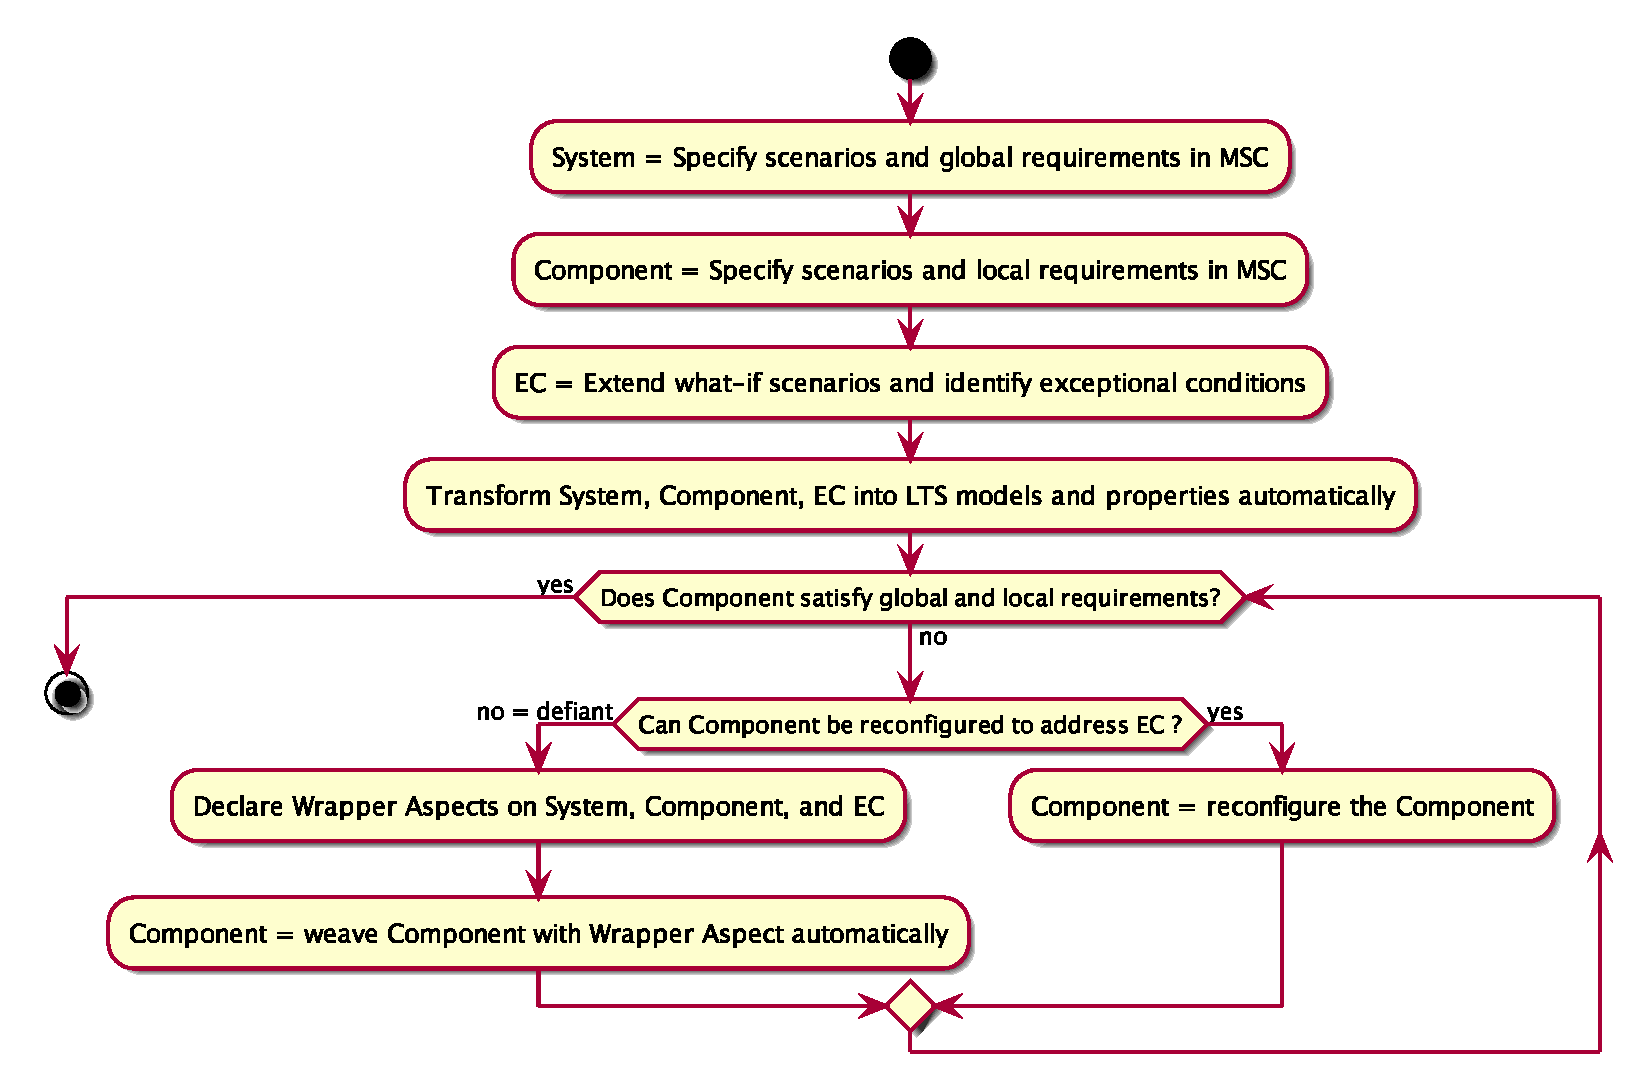
\includegraphics[width=0.9\columnwidth]{figures/activity.eps}
 \caption{Overview of the approach in an activity diagram}
 \label{fig:process}
 \vspace*{-0.5cm}
\end{figure}

%Our approach to cautious adaptation of a defiant component is explained below.


%illustrates the main constructs and relationships between the defiant component and the wrapper framework. The cautious adaptation weaving is responsible of 1) exposing the exceptional conditions of defiant component; 2) identifying the failure of the defiant component under the exceptional conditions; and 3) modifying the functionality of the defiant component to satisfy both exceptional and normal conditions. All these responsibilities can be defined as properties in the behaviour models that can be checked formally. 

%\begin{figure}[ht]
%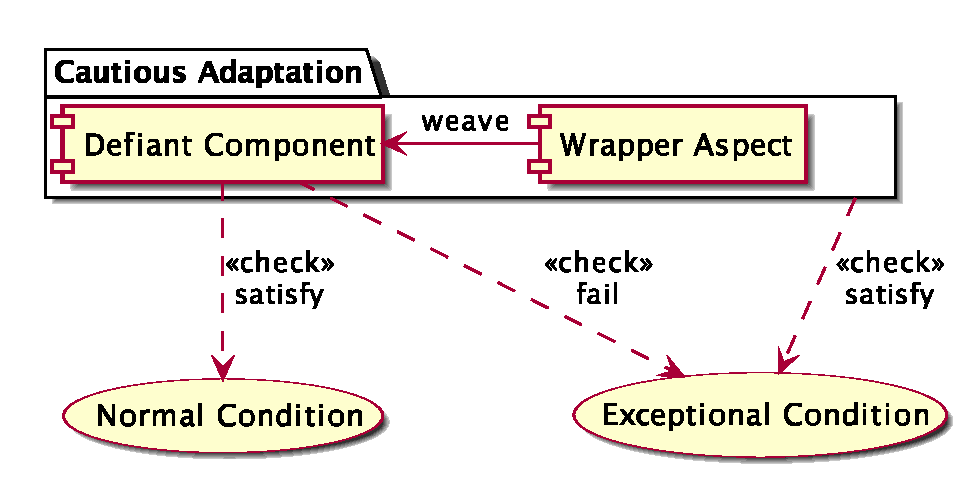
\includegraphics[width=\columnwidth]{figures/overview.eps}
%\caption{Overview of Cautious Adaptation Framework}\label{fig:overview}
%\vspace*{-1cm}
%\end{figure}

\subsection{Formalisation}

The general problem being tackled can be formalised using the semantics of Problem Frames~\cite{DBLP:books/daglib/0022946}, as follows. At the design time of a defiant component ($c$), given its world context ($W_c$), its specification ($S_c$) must satisfy its requirements ($R_c$), i.e., $W_c, S_c \models R_c$. 

%For instance, consider drone component $c$ with two requirements $R_c = R_1 \wedge R_2$, where $R_1$ is ``to fly from location $A$ to location $B$ when the battery level is above a threshold $\theta = 10\%$'' ($W_1$), and $R_2$ is ``to land safely when the battery level drops below $\theta$'' ($W_2 = \neg W_1$).

Suppose that component $c$ is being used as part of a system-of-systems ($s$). Based on the analysis of exception scenarios concerning a specific context of the system ($W_s$), which satisfies the condition $W_s \implies W_c$, component $c$ cannot satisfy global requirements of $s$. In other words, $W_s, S_s \not \models R_s$, where $S_s$ contains $S_c$. 

%In order to illustrate, consider the drone application scenario with an exceptional condition defined as $W_s = W_2 \wedge W_3 \wedge W_4$ where the battery level is below $\theta$ ($W_2$), but the battery level is sufficient to fly to location $B$ because of the wind condition ($W_3$), and it is flying above water by design of $S_s$ ($W_4$). According to the designed specification of the component $S_c$, the drone will land because of $W_2$, regardless of $W_3$, and the drone will land in the water because of $W_4$. The only feasible solution is to avoid safe landing in $W_s$, because if one rescues the landed drone from the water, it will be too late to replace it with another means of transportation even if the payload will not be damaged. Therefore, the problem is that it is not possible to change the specification of $S_c$. 

To verify that the wrapper executes its purpose, we formalise three conditions to be checked as follows:
\[
\begin{array}{ll}
W_s, S_s \not \models R_s & (\mbox{defiant identification})\\
W_s, S_s |_{c\rightarrow w(c)} \models R_s & (\mbox{defiant removal}) \\
W_c \setminus W_s, S_{w(c)} \models R_c & (\mbox{safety assurance})
\end{array}
\]
\begin{itemize}
\item Defiant identification checks that the component is defiant because its configurations do not satisfy global requirements.

\item Defiant removal checks that after wrapping up the defiant component with new behaviour, the global requirement can be restored in exceptional conditions.

\item Safety assurance checks that after wrapping up the defiant component with new behaviour, the local requirements are still satisfied in normal conditions. 
\end{itemize}

\subsection{Scenario Extensions on MSC}
To support the method, we extend the message sequence chart (MSC) specification with an operator (o) to represent an \textit{interception point} in which exceptional scenarios can be plugged to wrap the defiant component. Several exceptional behaviours can be plugged in the same interception point, indicating other possible behaviours according to alternative contexts. If there is no exceptional scenario plugged in an interception point, the expected default behaviour is performed.

Figure~\ref{fig:drone_msc} shows part of high-level message sequence charts (hMSC) specification for the payload organ delivery scenario discussed in Section 1. Each box in the hMSC corresponds to a basic message sequence chart (bMSC), like UML sequence diagrams, exchanging messages between different entities, whilst the bMSC are put together through control flows (branches and loops). Figure~\ref{fig:drone_bmsc} depicts the referred bMSCs for part of the drone payload delivery example.   
% Need one example bMSC. 

\begin{figure}
    \includegraphics[width=\columnwidth]{figures/new_drone_msc.png}
    \caption{hMSCs for the drone scenario}
    \label{fig:drone_msc}
    \vspace*{-0.25cm}
\end{figure}

\begin{figure}
    \includegraphics[width=\columnwidth]{figures/new_drone_bmsc.png}
    \caption{bMSCs for the drone delivery scenario}
    \label{fig:drone_bmsc}
    \vspace*{-0.5cm}
\end{figure}

In Figure~\ref{fig:drone_msc}, the predefined scenarios are represented by a full rectangle and are part of the normal specification of a drone, while the exceptions are represented by dashed rectangles. As shown in Figure~\ref{fig:drone_msc}, through a controller the pilot can control the drone to take off, and can manoeuvre the drone when the battery is above a certain threshold $\theta = 10\%$, while it has not reached the destination. When the pilot sends a landing command to the drone, this is acknowledged when the drone lands in the ground.  During a flight, a drone periodically checks the status of its internal devices such as battery level and distance from the destination, represented by \textit{b} and \textit{d}, respectively, in the guard conditions over the transitions. In the example, if the battery level is above the expected threshold and the drone is not yet in its destination, the drone keeps flying. If the drone reaches its destination, it performs a landing action. If the battery is below the expected threshold, the drone performs a safe landing in accordance to its predefined specification. 

The exceptional conditions added in the interception point state that if the distance to the expected destination is less than 2km, the drone is flying over the river (condition \textit{on\_water==true}), and the wind is strong (condition \textit{wind==strong}), then the pilot can keep the drone flying even in a low-level battery situation and then land, thus being able to complete its overall goal (delivering the medical payload) successfully. Nonetheless, if the battery is low, the drone is above water, but the drone is more than 2km away or the wind is not strong,
% Paolo: Fig 2 needs update
% "[d > 2]" => "[d > 2 || wind!=strong]"
then the action is to move the drone aside in order to land it on the ground. 

% Figure~\ref{fig:overview} shows an overview of the relationship between the defiant component and the wrapper technique. The cautious adaptation approach is responsible to: (i) expose exceptional conditions of defiant components; (ii) identify failure of  defiant components under the exceptional conditions; and (iii) modify the functionality of defiant components to satisfy both exceptional and normal conditions. All these responsibilities can be defined as properties in behaviour models that can be checked formally. 

\subsection{The Wrapper Aspect}
The introduction of a {\it wrapper} $w(c)$ changes the defiant behaviour of the component $c$, i.e. $W_s, S_{w(c)} \not \models R_c$, retaining the essential satisfaction of global requirements when $c$ is substituted with $w(c)$:  $W_s, S'_s \models R_s$ where $S'_s = S_s |_{c \rightarrow w(c)}$. Furthermore, the adaptation is {\it cautious} because other than the exceptional condition $W_s$, the wrapped component should still behave like the original designed component, i.e., $(W_c \setminus W_s), S_{w(c)} \models R_c$. 

%\subsubsection{A Wrapper by Aspect-Orientation}
Based on aspect-oriented programming (AOP)~\cite{Kiczales:2001}, we introduce wrappers that can achieve the above requirements. The exceptional conditions identified in the scenarios provide an indication where changes in the system should occur ({\it joint points}). Once the join points are identified, we represent them as regular expressions as {\it point-cuts}, so that a replacement of the behaviour after the join points can be done through aspect {\it advices}. Aspect advices are exceptionally handled, which can invoke existing functionalities of original components, but can also introduce additional functions and conditions that do not exist in the original components.

%Since a component at design time is unaware of its future exceptional usage, it will not be able to expose its full implementation to the system integrator. Fortunately, {\it aspect-oriented} framework can intercept the control flow of the behavioural specification~\cite{Xu07}. 

%For example, to identify the join points, i.e., where  modifications are allowed to change. Methodologically, the exceptional conditions we obtain from the exceptional scenarios provide us a clue where such join points can be.

%Once the join points are identified, we can use regular expressions to express them as {\it point-cuts} so that a replacement of the behaviour after the join points can be done through aspect {\it advices}. Aspect advices in this situation are exceptional handling which can still invoke existing functionality of the original components, but can also introduce additional functions and conditions that do not exist in the original component. But the weaving of the aspect-oriented wrapper must be performed with caution. 

In the situation in which there are more than one wrapper for the same exceptional condition, to avoid interference~\cite{Katz:2008:IAI:1394496.1394500}, we define a precedence order among wrappers. For example, a safety wrapper is regarded with a high-level of importance and should be applied afterwards, to override applied unsafe wrappers. 
